% MAIN.TEX - University of Warwick, Integrated Science, Report
% Template by Andrew Blanks and Stephen Royle
%%%%%%%%%%%%%%%%%%%%%%%%%%%%%%%%%%%%%%%

% PREAMBLE
\documentclass[11pt,a4paper]{article}
\usepackage[utf8]{inputenc} % text encoding, for special characters e.g. umlauts use \"
\usepackage{amsmath} % for equations
\usepackage{amsfonts} % for equations
\usepackage{amssymb} % for equations
\usepackage{graphicx} % for figures
\usepackage{wrapfig} % for figures
\usepackage[final]{pdfpages}
\usepackage[margin=2cm]{geometry}
\usepackage{authblk}
\usepackage[authoryear,round]{natbib}
\usepackage{siunitx} % for correct units e.g. 10 nm is \SI{10}{\nano\metre}
\DeclareSIUnit\Molar{\textsc{m}} % formats Molar concentrations e.g. \SI{1}{\micro\Molar}
\usepackage[version=4]{mhchem} % for chemical entities e.g. \ce{FeSO4}
\usepackage[font=small,labelfont=bf]{caption} % caption/legends for figures
\usepackage{parskip} % controls gap between paragraph and previous
\usepackage{titlesec} % controls titles and sections
\usepackage{lipsum}
\usepackage[hidelinks]{hyperref} % makes links clickable

% provide details of your project report
\title{Declarative title of my report}
\author{Alex Smith\thanks{Corresponding author: a.smith@warwick.ac.uk}}
\affil{Integrated Science, University of Warwick, Gibbet Hill Road, Coventry, CV4 7AL, UK}
\date{} % add the date here

%%%%%%%%%%%%%%%%%%%%%%%%%%%%%%%%%%%%%%%

\begin{document}

\maketitle

\begin{abstract}
Abstract of the paper goes here.
\lipsum[1]
\end{abstract}

% the * after section prevents numbering
\section*{Introduction}

Introduction text goes here.
\lipsum{2-6}
Text is added like this.
This is a reference to a published paper \citep{watson_molecular_1953}.
We can cite other things too \citep{tipton_complexities_2019,zheng_genome_2011,alberts_molecular_2002}

\section*{Materials and Methods}

\subsection*{Materials} 
Materials text goes here.
\lipsum[3]
 
\subsection*{Method1}  
Method 1 text goes here.
\lipsum[3]

\subsection*{Method2}
Method 2 text goes here.
\lipsum[3]

\subsection*{Data analysis}
Data analysis section goes here.
\lipsum[3]




% figure goes here but can be moved to wherever it looks best
\begin{figure}
     \centering
     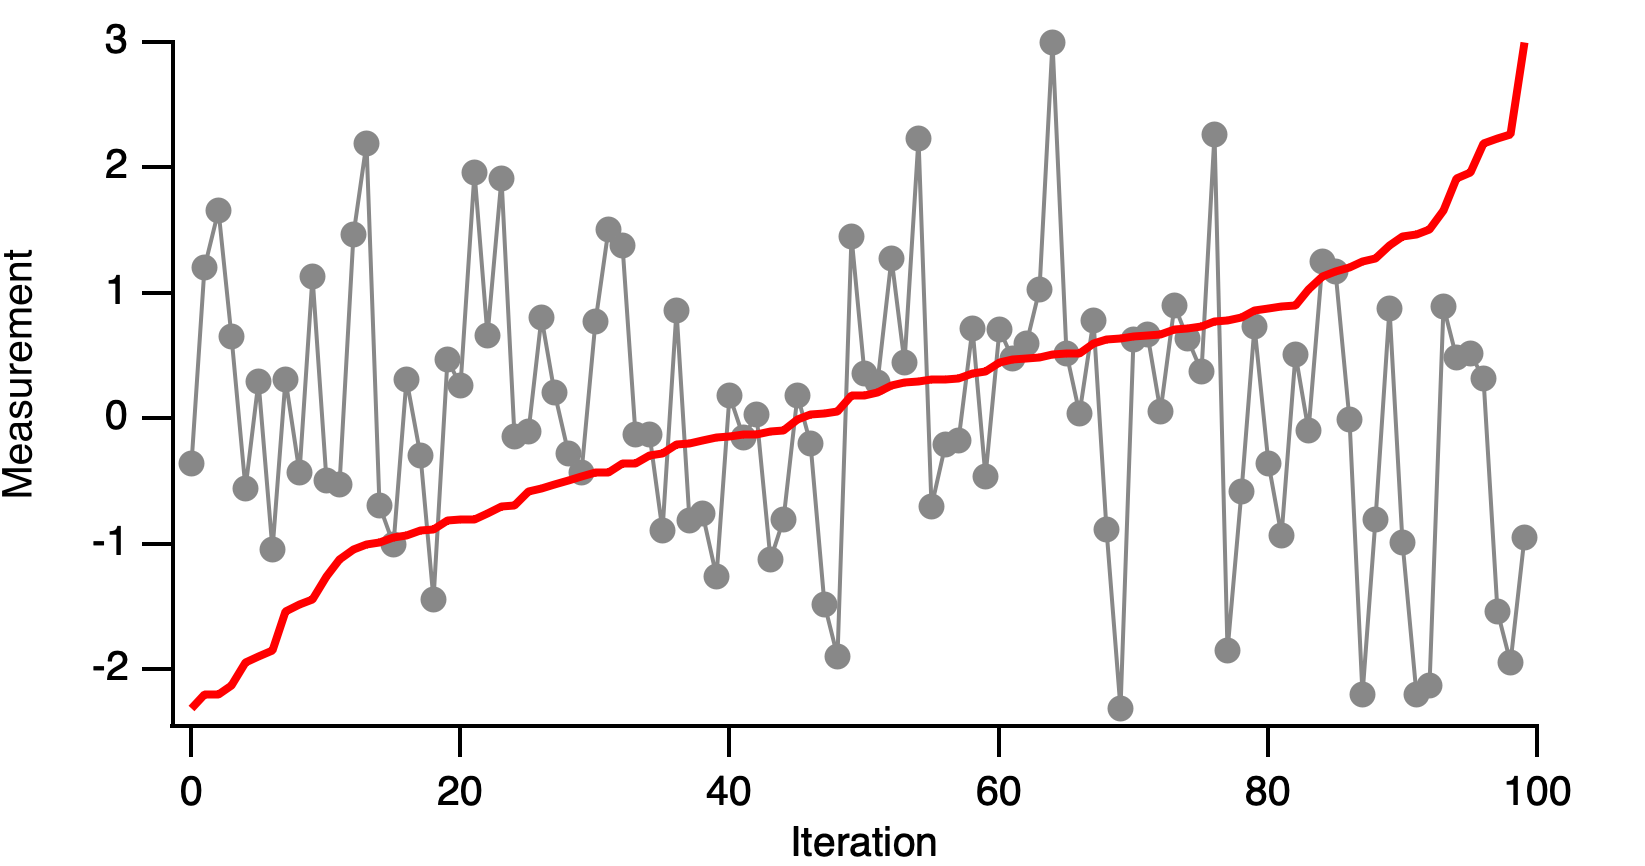
\includegraphics[width=10cm]{Fig_1}
        \caption{
                \textbf{A}:~Blah
                \textbf{B}:~Blah
                \textbf{C}:~Blah
                \textbf{D}:~Blah
        }
        \label{fig:1}
\end{figure}

\section*{Results}

Results text goes here 
% reference figure 1 by
(Fig.~\ref{fig:1}).
\subsection*{Blah}
Subsection of results Blah goes here


\section*{Discussion}

Text of discussion goes here
\lipsum{12-15}


\section*{Conclusion}

Conclusion text goes here.
\lipsum[5]


\section*{Acknowledgments}

Acknowledgments go here.

\newpage
\bibliographystyle{modabbrv}
\bibliography{refs.bib}

\end{document}